\documentclass[runningheads,a4paper]{llncs}

\usepackage{amssymb}
\setcounter{tocdepth}{3}
\usepackage{graphicx}
\usepackage{array}

\usepackage{url}
\urldef{\mailsa}\path|abdulfatirs@gmail.com, abdulfatir@outlook.com|
\newcommand{\keywords}[1]{\par\addvspace\baselineskip
\noindent\keywordname\enspace\ignorespaces#1}
\newcommand{\interests}[1]{\par\addvspace\baselineskip
\noindent \textbf{Interests:}\enspace\ignorespaces#1}
\usepackage[usenames, dvipsnames]{color}

\definecolor{azure}{RGB}{0, 7, 255}


\usepackage{hyperref}
\hypersetup{
    colorlinks=true,
    linkcolor=blue,
    filecolor=magenta,      
    urlcolor=azure,
}
\graphicspath{{images/}}

\begin{document}

\mainmatter  % start of an individual contribution

% first the title is needed
\title{GSoC 2016 Proposal \\ Blood Sample Image Analysis}

% a short form should be given in case it is too long for the running head
\titlerunning{Blood Sample Image Analysis}

\author{Abdul Fatir Ansari}
%
\authorrunning{Blood Sample Image Analysis}

\institute{Department of Civil Engineering, IIT Roorkee, India, PIN 247667 \\ \mailsa \\ \url{http://abdulfatir.com}}

\maketitle

\interests{Computer Vision, Image Processing, Machine Learning, Cryptography, Bioinformatics}

\begin{abstract}
The aim of this project is to use the camera and processing power of modern day cell phones to develop an intuitive and user-friendly application for the detection of cancer biomarkers from a small drop of blood. This will serve as a screening test for the same. The application will allow the user to take images of the blood samples in a set format. The image will then be segmented using a background subtraction algorithm to detect the regions of interest. After noise removal, the intensity of each individual blob will be calculated. A linear curve will be fit through the intensity and known concentration data and the concentrations of the unknown samples will be estimated from the standard curve which will quantify the various molecules present in the sample.
\keywords{Image Analysis, Segmentation, Cancer, Biomarker, Android, Java, OpenCV}
\end{abstract}

\section{Background}

I'm currently in junior year of civil engineering at \emph{Indian Institute of Technology, Roorkee}. I've been involved in programming for 7 years now, of which the last 2 have been in the fields of Computer Vision \& Machine Learning. I'm an ardent follower of the advancements in the field of Artificial Intelligence and am always eager to contribute to the field. Image Processing \& Computer Vision form a very important part of AI Research and hence this project interests me.

\subsection{Image Processing \& Computer Vision}

I've worked on various projects involving computer vision and image processing some of which include the following.

\begin{enumerate}

\item \textbf{Posture Recognition in HINE Exercises} -- A multi-class classification task which involved segmentation of infant's body from videos of Hammersmith Infant Neurological Examinations, post-processing the segmented videos, skeletonization, and then feature extraction to train a Hidden Markov Model for broad level exercise classification.  \\
\textbf{\emph{Languages}}: C++ (OpenCV), Python, MATLAB \\
\textbf{\emph{Publication}}: A. F. Ansari, P. P. Roy, and D. P. Dogra. Posture recognition in HINE exercises. \emph{Proceedings of International Conference on Computer Vision and Image Processing}, 2016 (in press). \\
\textbf{\emph{Current Work}}: Finer level sequence labelling using Bag of Words approach and training Recurrent Neural Networks (LSTM) for the problem of classification.
\item \textbf{Vehicle Detection \& Tracking} -- A vehicle detection and tracking task for estimation of traffic flow parameters on an unsignalized intersection. \\
\textbf{\emph{Languages}}: C++ (OpenCV)

\end{enumerate}

\subsection{Android}

I've been working on Android platform for 3 years now. The following two applications among others showcase my work in this field.

\begin{enumerate}
\item \textbf{Sanibridge Health App} (\emph{ongoing}) -- An Android health application for monitoring various biomarkers. I worked on the full stack development of the application including the backend under the supervision of Dr. Tomas Helikar. \\
\textbf{\emph{Languages}}: Java (Android), PHP+MySQL
\item \textbf{Dodgy Bat} -- An obstacle avoidance game for Android platform using LibGDX. \\
\textbf{\emph{Languages}}: Java (Android)

\end{enumerate}

\section{Programming Skills}

\begin{itemize}
\item Java, Python, C++, MATLAB are the languages I'm most experienced with. I'm also well acquainted with web development both backend (PHP, Python, NodeJS), DBMS (MySQL), and frontend (HTML+CSS+JS and their various frameworks). 
\item I am also familiar with C\#, Perl and \LaTeX.
\item I've been working on Open Source projects since 2010. Some of my projects are also on \href{https://github.com/abdulfatir}{GitHub}.
\item I want to learn and build new image processing and computer vision algorithms, and learn about the applications of machine learning in computer vision this summer.
\end{itemize}

\section{Biology}

I'd studied biology at high school level. I am interested in learning biology this summer because I've been working in the field of medical computer vision of late and the knowledge of biology related to the work I am doing will be a plus.

\section{Details of Proposal Challenge}

I used the following algorithm for the proposal challenge in \href{https://www.dropbox.com/sh/xfpl8xw6l91yubo/AACRVdraU5jr7qRxJeZAv1hpa?dl=0}{Python \& C++}. 

\subsection{Methodology}

\begin{enumerate}

\item Convert the image into HSV color space and threshold the image based on the presence of red hue. (Circular Hough Transform after finding edges (Canny) of the image can also be used for blob detection)
\item Remove noise and false detections using 5x5 median filter and morphological operations.
\item Detect the contours of the segmented image and keep the largest ones (which represent the samples) and discard small blobs (if present) as spurious detections.
\item For each blob, calculate the average pixel intensity value after converting the image into grayscale.
\item Input the concentration of known blobs and fit a one-degree curve through the data (since the Standard Curve is linear).
\item Find the values of concentrations of unknown sample and quality control samples from the plot.
\end{enumerate}
\subsection{Results}

The results of calculations on PC and Android platform are given in tables \ref{table:pcresults} and \ref{table:andresults} respectively.

\begin{table}
\begin{center}
\setlength\tabcolsep{2.5pt}
\def\arraystretch{1.5}
\begin{tabular}{| m{5em} m{7em} m{9em} m{5em} |}
\hline
Sample & Actual Value & Calculated Value & Error\\
\hline
\hline
QC1 & 156 ng/ml & 149.82 ng/ml & 3.9 \%\\
\hline
QC2 & 750 ng/ml & 843.15 ng/ml & 12.4 \%\\
\hline
Unknown Sample & NA & 273.41 ng/ml & NA \\
\hline
\end{tabular}
\\
\caption{Results on PC}
\label{table:pcresults}
\textbf{ D = 0.05081 C + 75.55\\}
D = Darkness (255-Brightness) \\ C = Concentration in ng/ml
\end{center}
\end{table}

\begin{table}[h!]
\begin{center}
\setlength\tabcolsep{2.5pt}
\def\arraystretch{1.5}
\begin{tabular}{| m{5em} m{7em} m{9em} m{5em} |}
\hline
Sample & Actual Value & Calculated Value & Error\\
\hline
\hline
QC1 & 156 ng/ml & 151.82 ng/ml & 2.68 \%\\
\hline
QC2 & 750 ng/ml & 847.86 ng/ml & 13.05 \%\\
\hline
Unknown Sample & NA & 270.80 ng/ml & NA \\
\hline
\end{tabular}
\\
\caption{Results on Android Device}
\label{table:andresults}
\end{center}
\end{table}

\begin{figure}[h]
\begin{center}
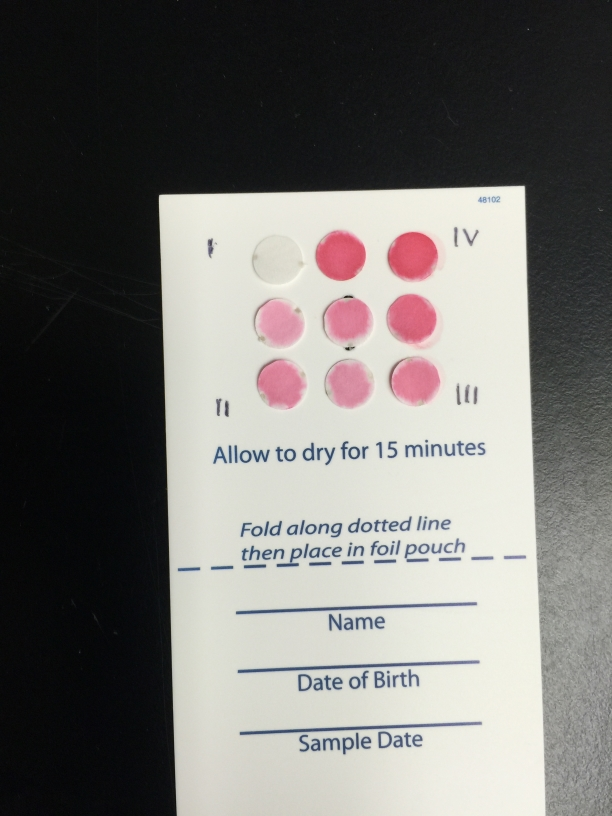
\includegraphics[scale=0.18]{in}
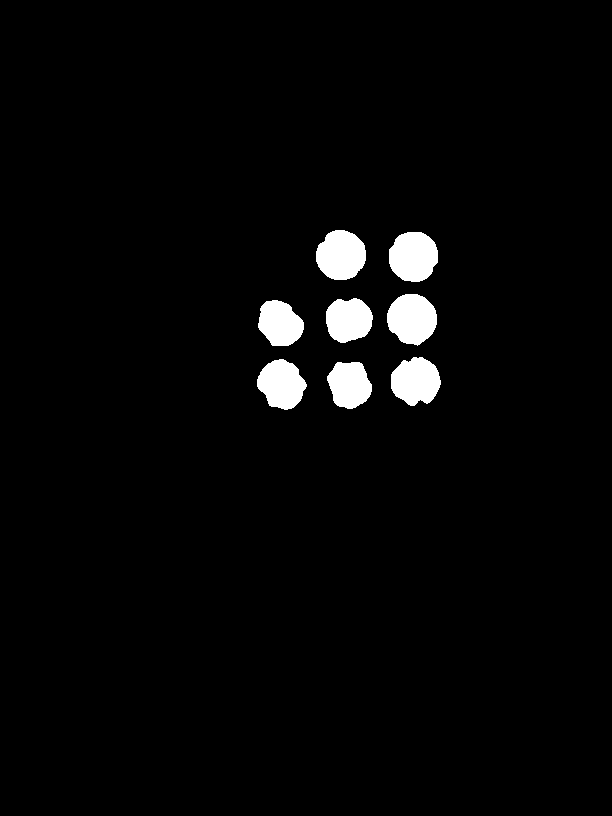
\includegraphics[scale=0.18]{out_2}
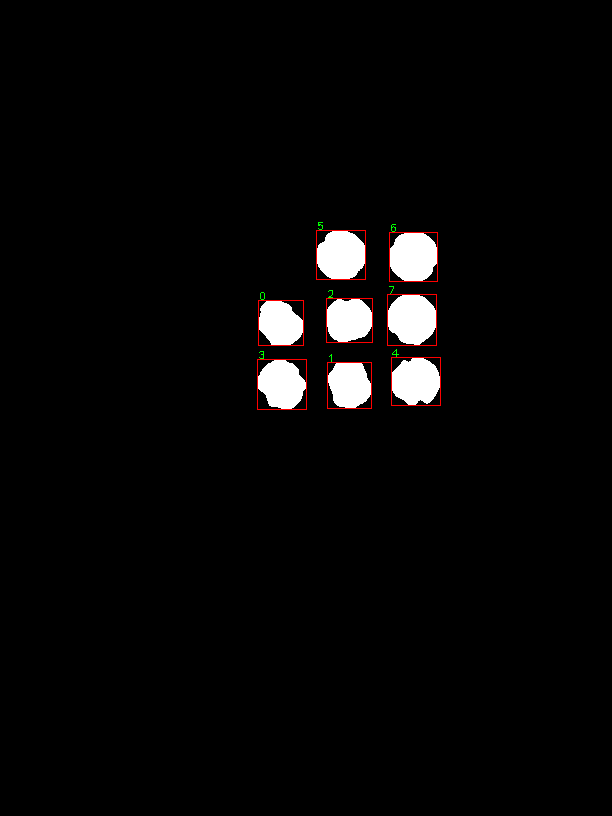
\includegraphics[scale=0.18]{out_3}
\caption{Input $\rightarrow$ Segmentation \& Noise Removal $\rightarrow$ Blob Detection }
\end{center}
\end{figure}

\begin{figure}[h!]
\begin{center}
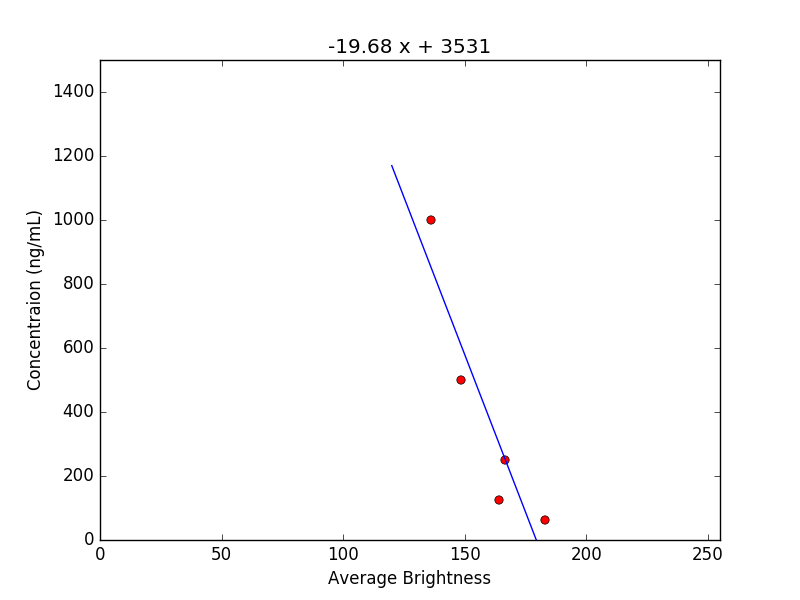
\includegraphics[scale=0.23]{raw}
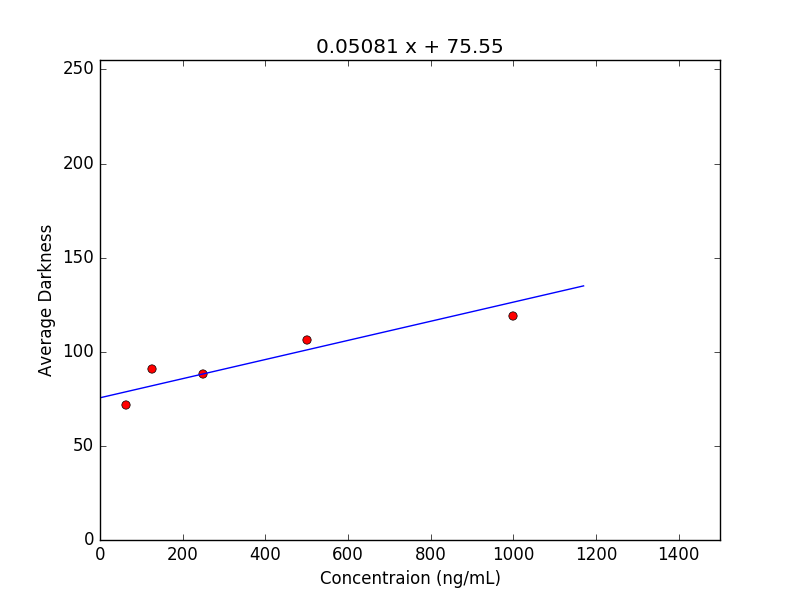
\includegraphics[scale=0.23]{stand}
\caption{Raw Curve \& Standard Curve}
\end{center}
\end{figure}

\subsection{Android Prototype}

I also developed an Android Prototype (code on GitHub \href{https://github.com/abdulfatir/Blood-Analysis}{repository} and fully functional code and binaries \href{https://www.dropbox.com/sh/gge2q46ww5nw5zy/AABBIoVO_r9iy__i5pFRjzsMa?dl=0}{here}) for the above algorithm. The video of the workflow can be found \href{https://www.youtube.com/watch?v=ReJSvmJ23z0}{here}. The special feature of this prototype application is that I've made it interactive \emph{i.e.} one can tap on the detected blobs and edit the properties of that very sample.
\\ \\
\newpage
\emph{\textbf{Usage}}
\begin{enumerate}
\item Tap Load Image and look for the image in the gallery.
\item Tap Analyze and wait. The app will look for 8 largest red hue blobs and will outline them with red color and label them with a number.
\item Tap on each rectangle to input values for that blob.
\item An input dialog will open which will ask for Sample Type and Concentration.
\begin{itemize}
\item For Known samples, choose Known and enter concentration.
\item For Quality Control samples, choose QualityControl and enter concentration.
\item For Unknown sample, choose Unknown and leave concentration as it is.
\end{itemize}
\item Tap Results and a dialog box with results and equation will be shown.
\end{enumerate}

The screenshots of the Android application are shown in figures \ref{fig:scr1}, \ref{fig:scr2} and \ref{fig:scr3}.

\begin{figure}[h!]
\begin{center}
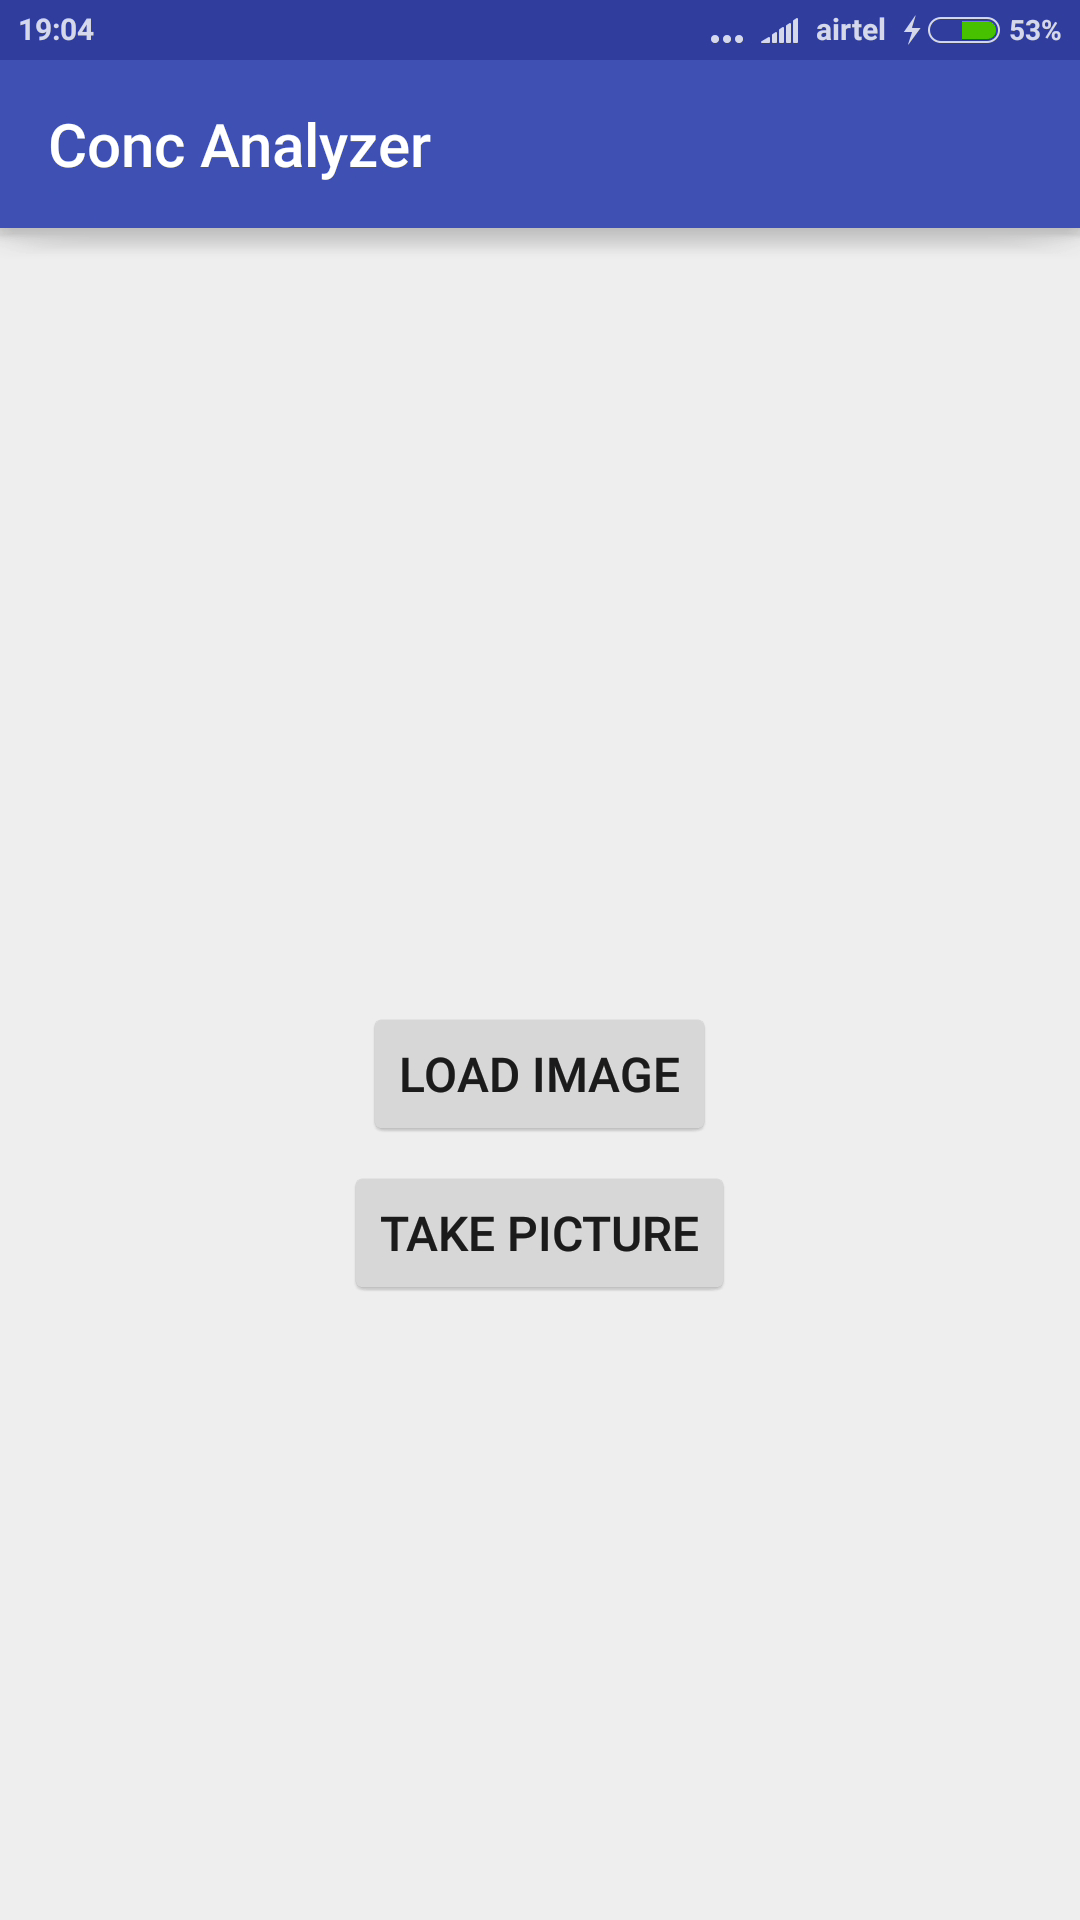
\includegraphics[scale=0.12]{conc1}
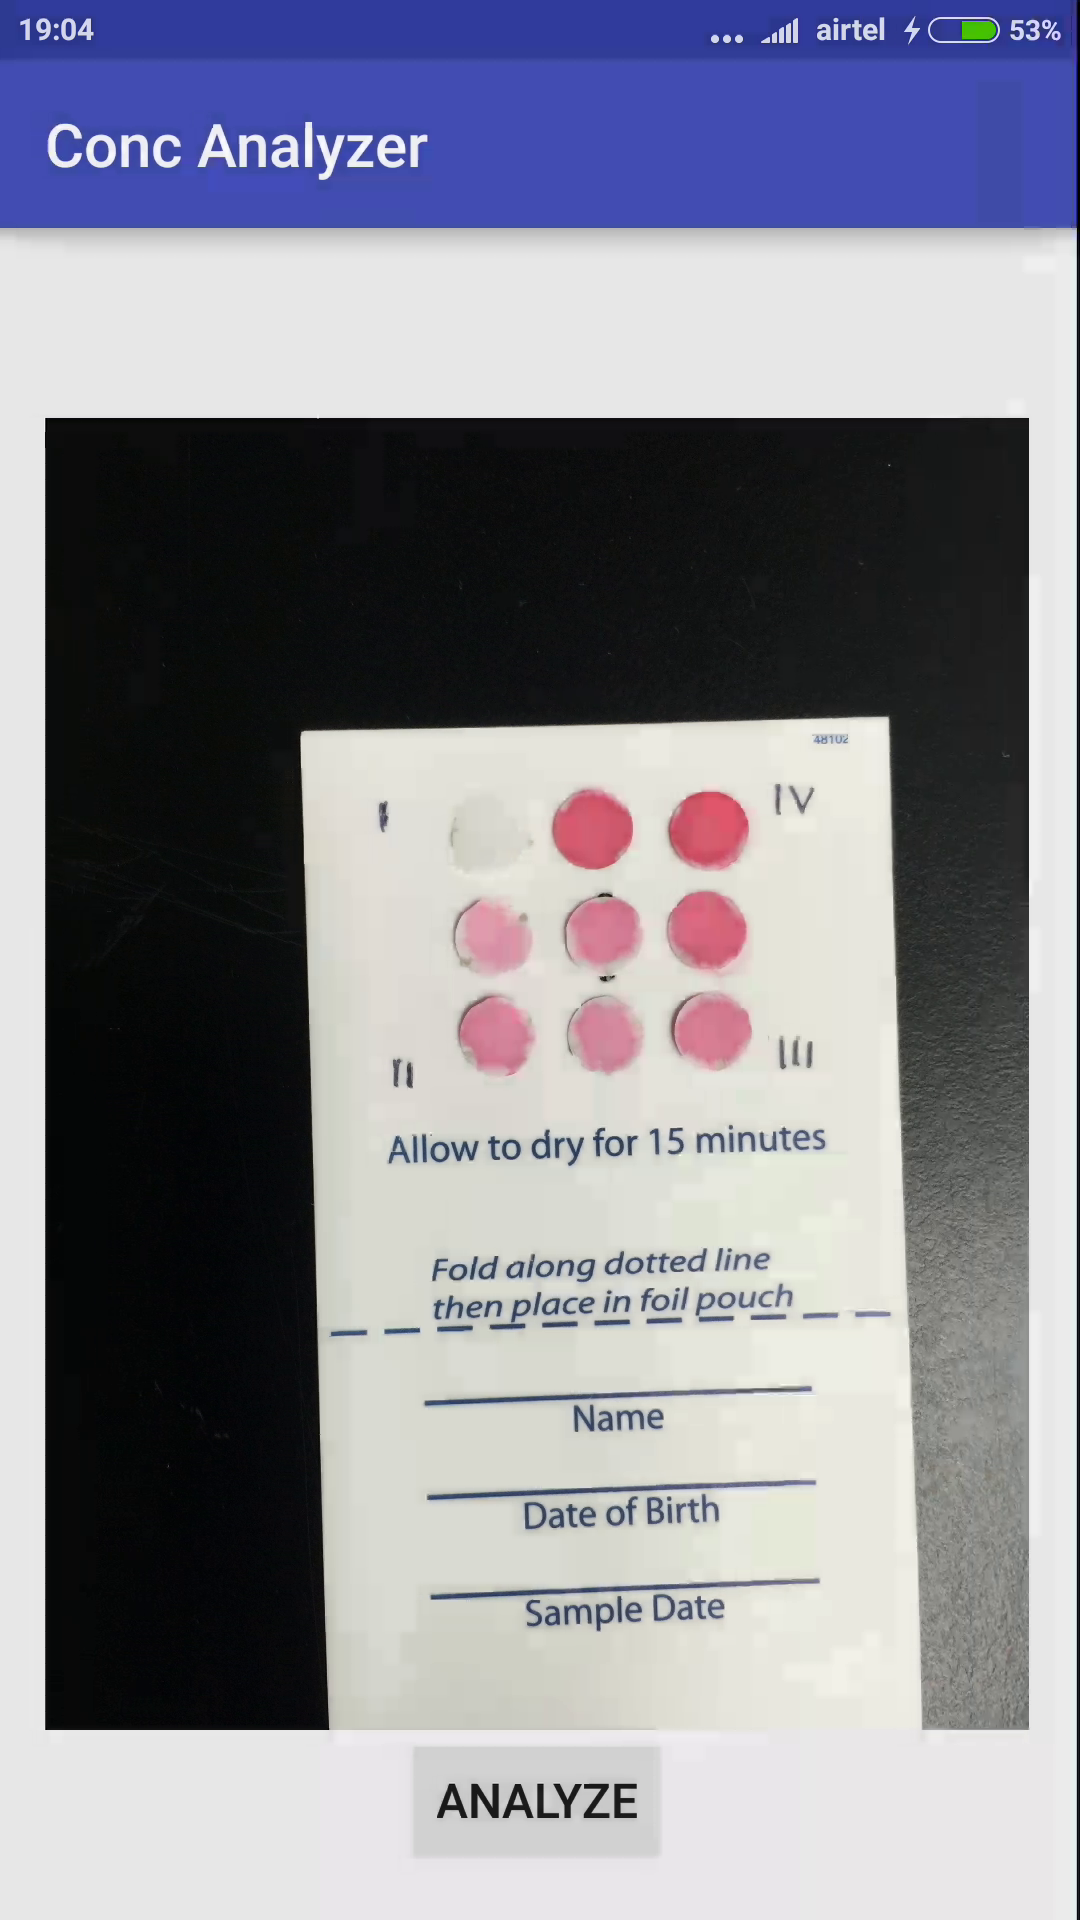
\includegraphics[scale=0.12]{conc2}
\caption{Home Screen \& Analyze Screen}
\label{fig:scr1}
\end{center}
\end{figure}

\begin{figure}[h!]
\begin{center}
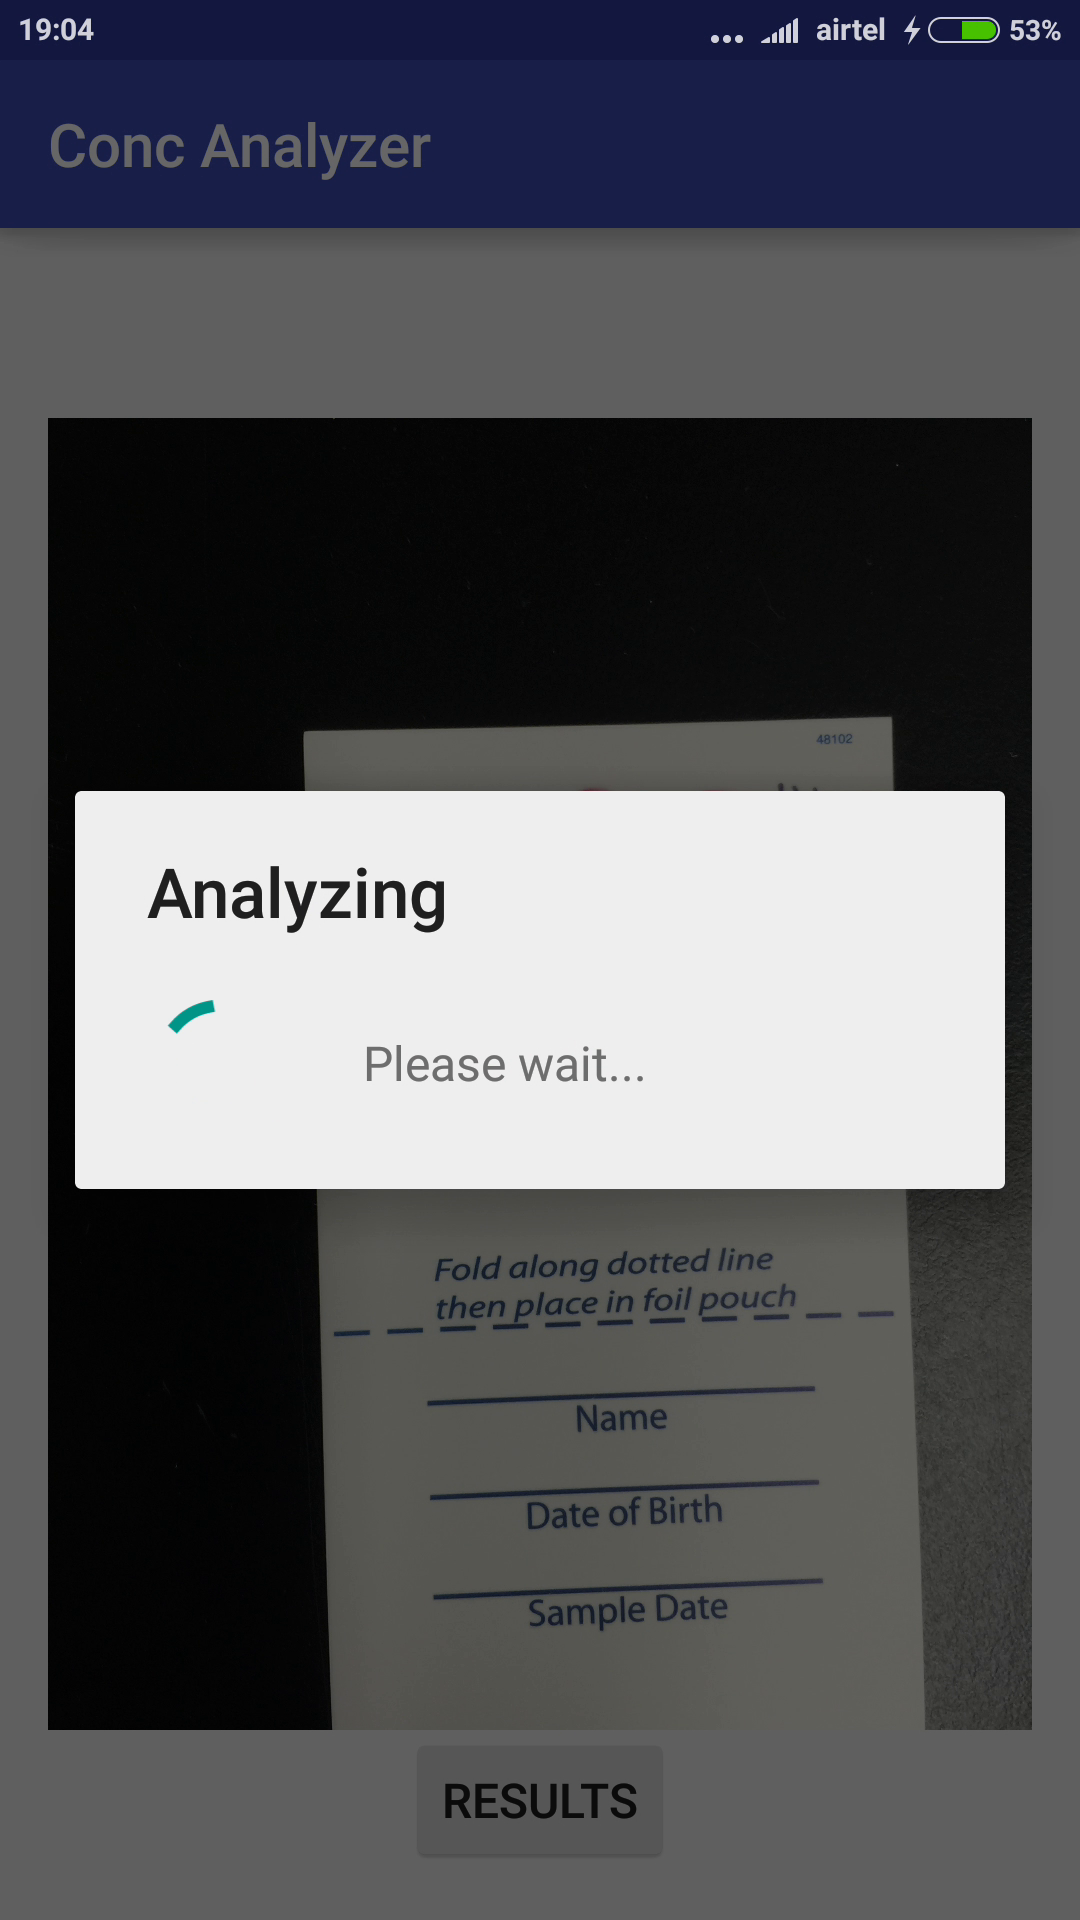
\includegraphics[scale=0.12]{conc3}
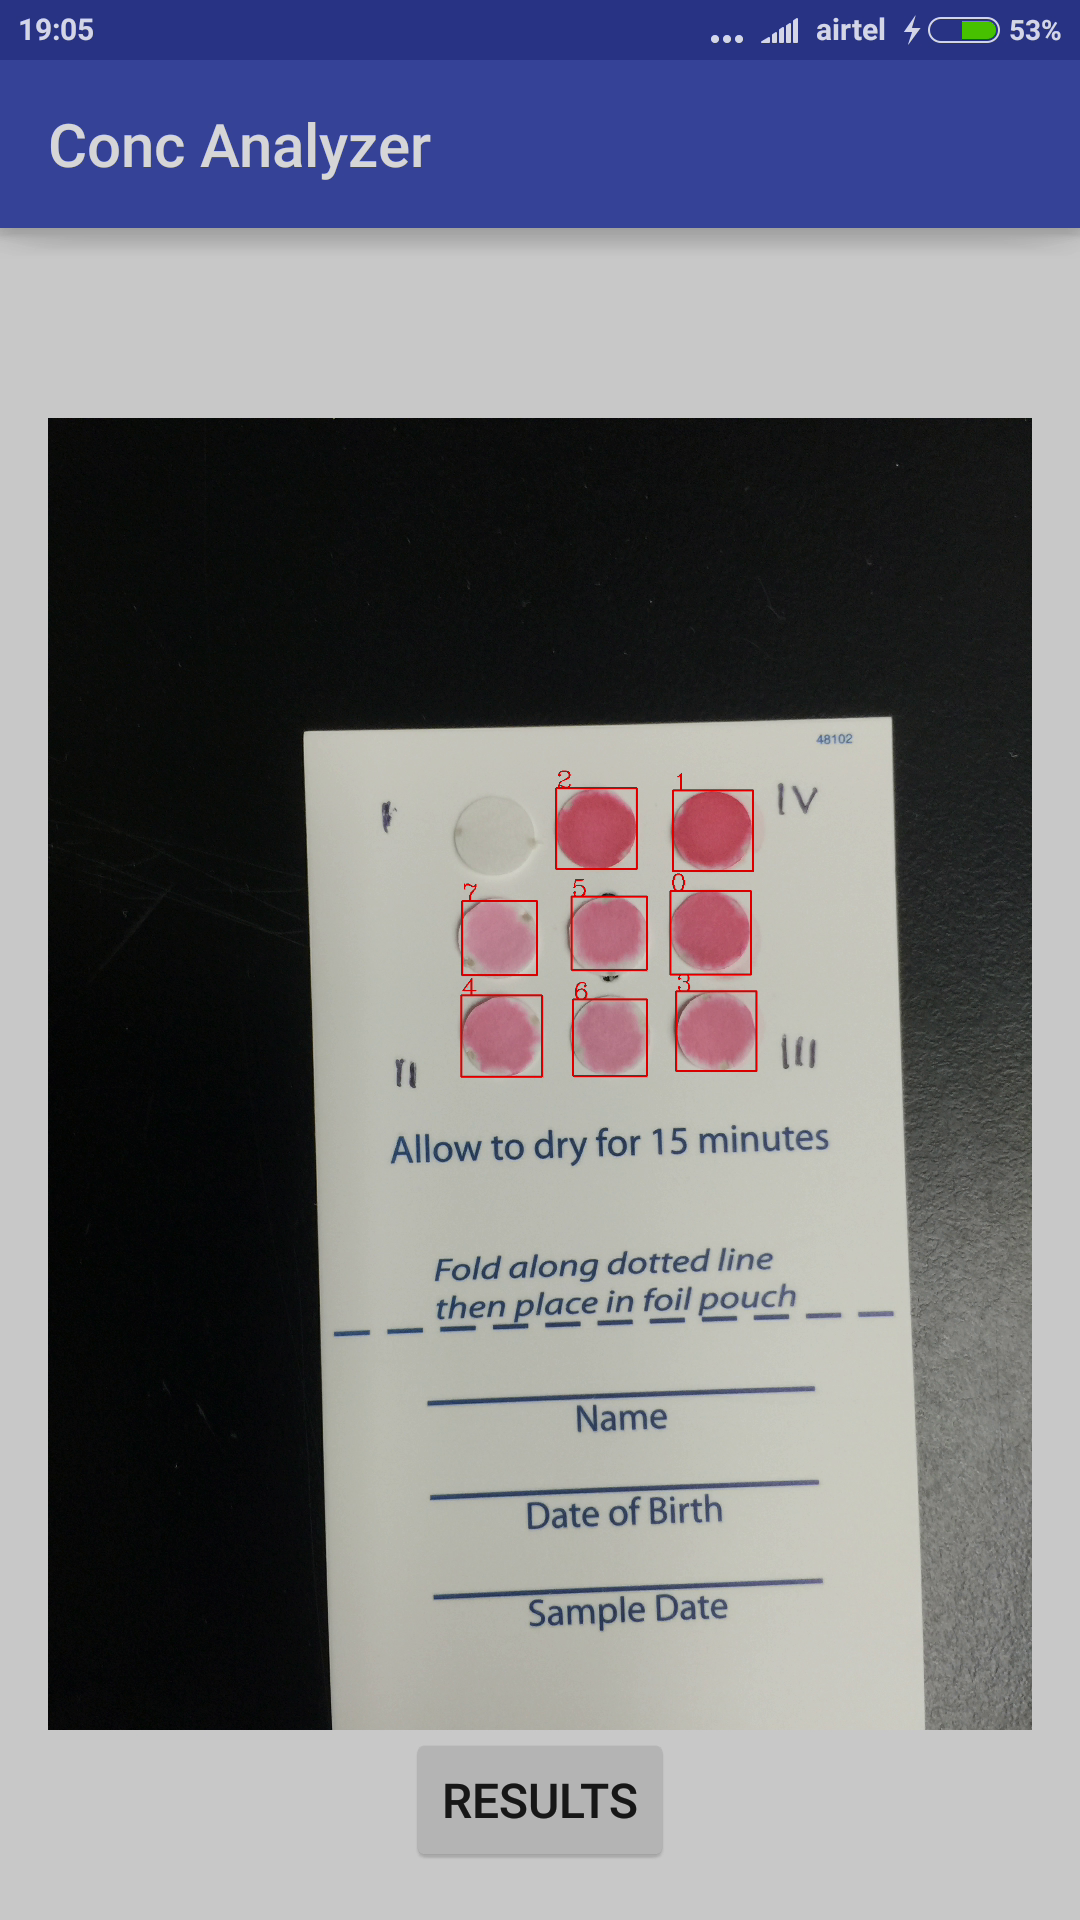
\includegraphics[scale=0.12]{conc4}
\caption{Analyzing \& Detected Blobs}
\label{fig:scr2}
\end{center}
\end{figure}

\begin{figure}[h!]
\begin{center}
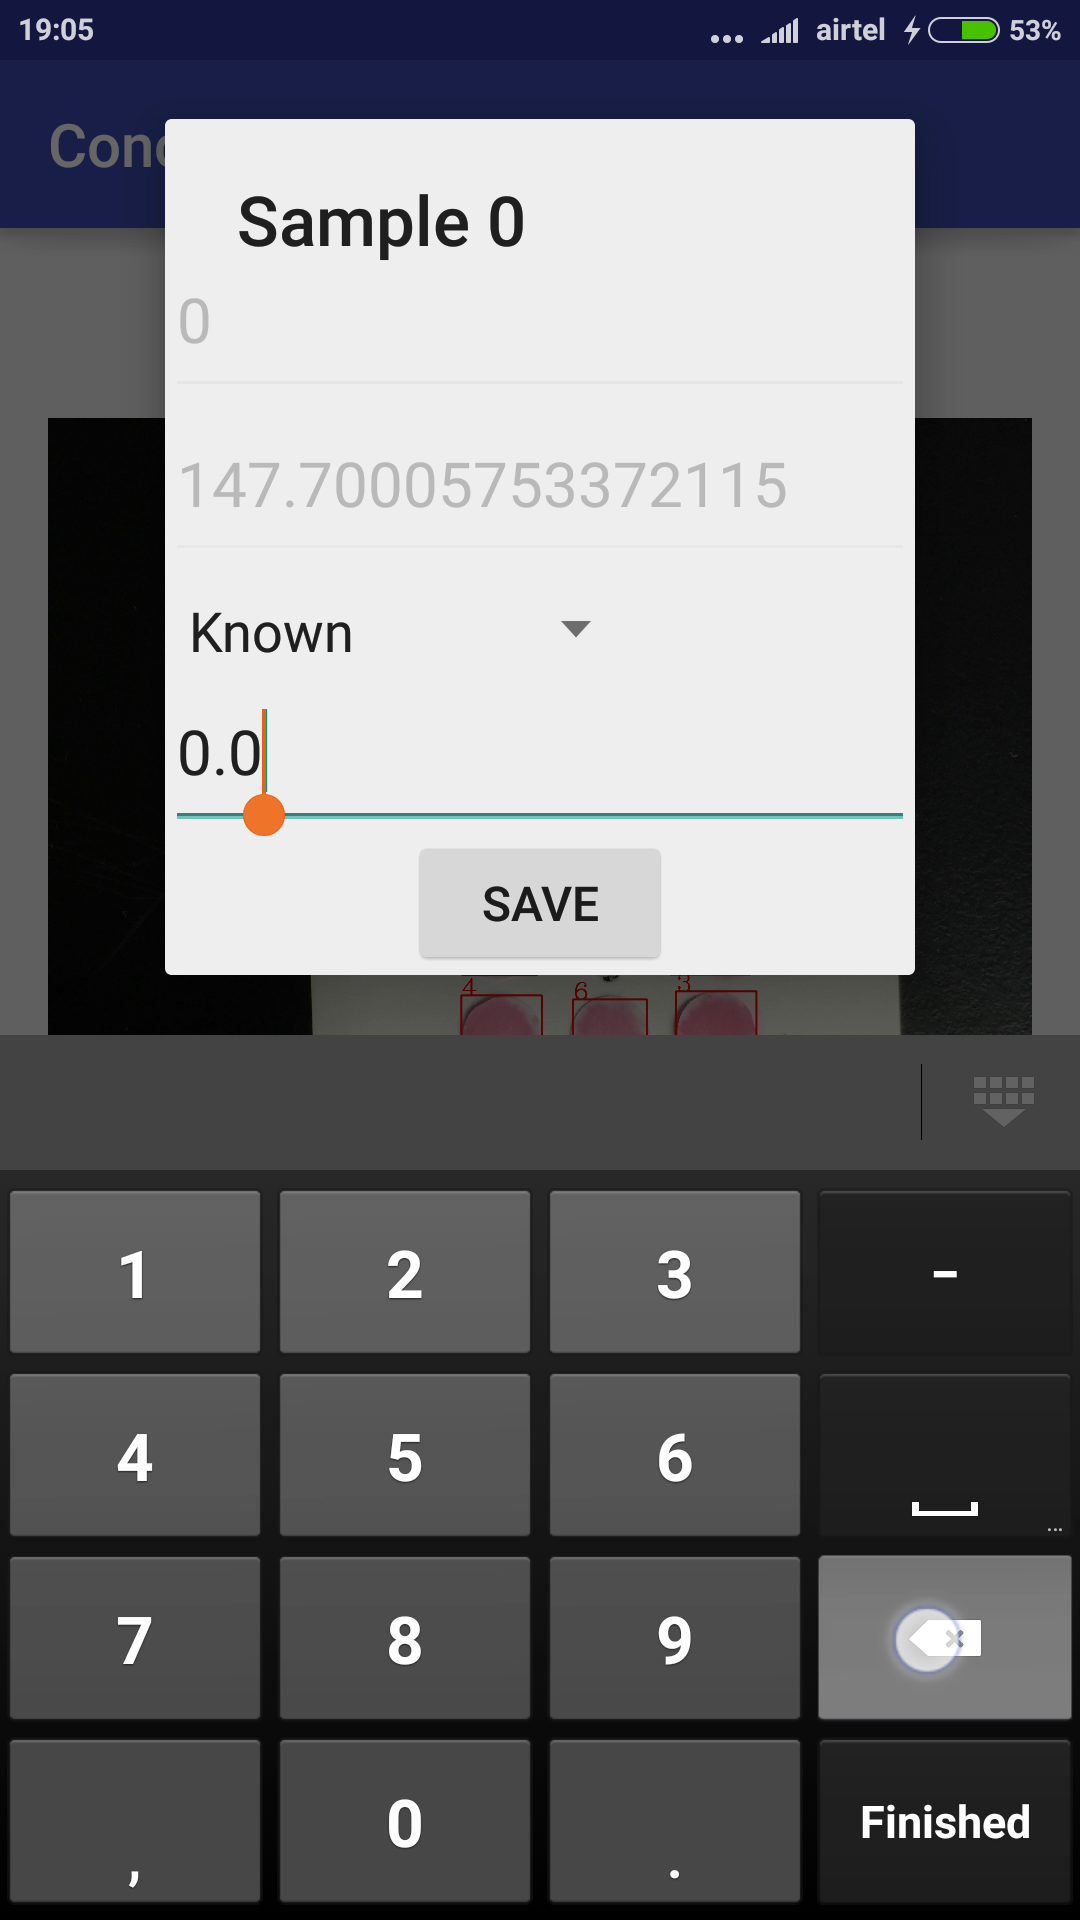
\includegraphics[scale=0.11]{conc5}
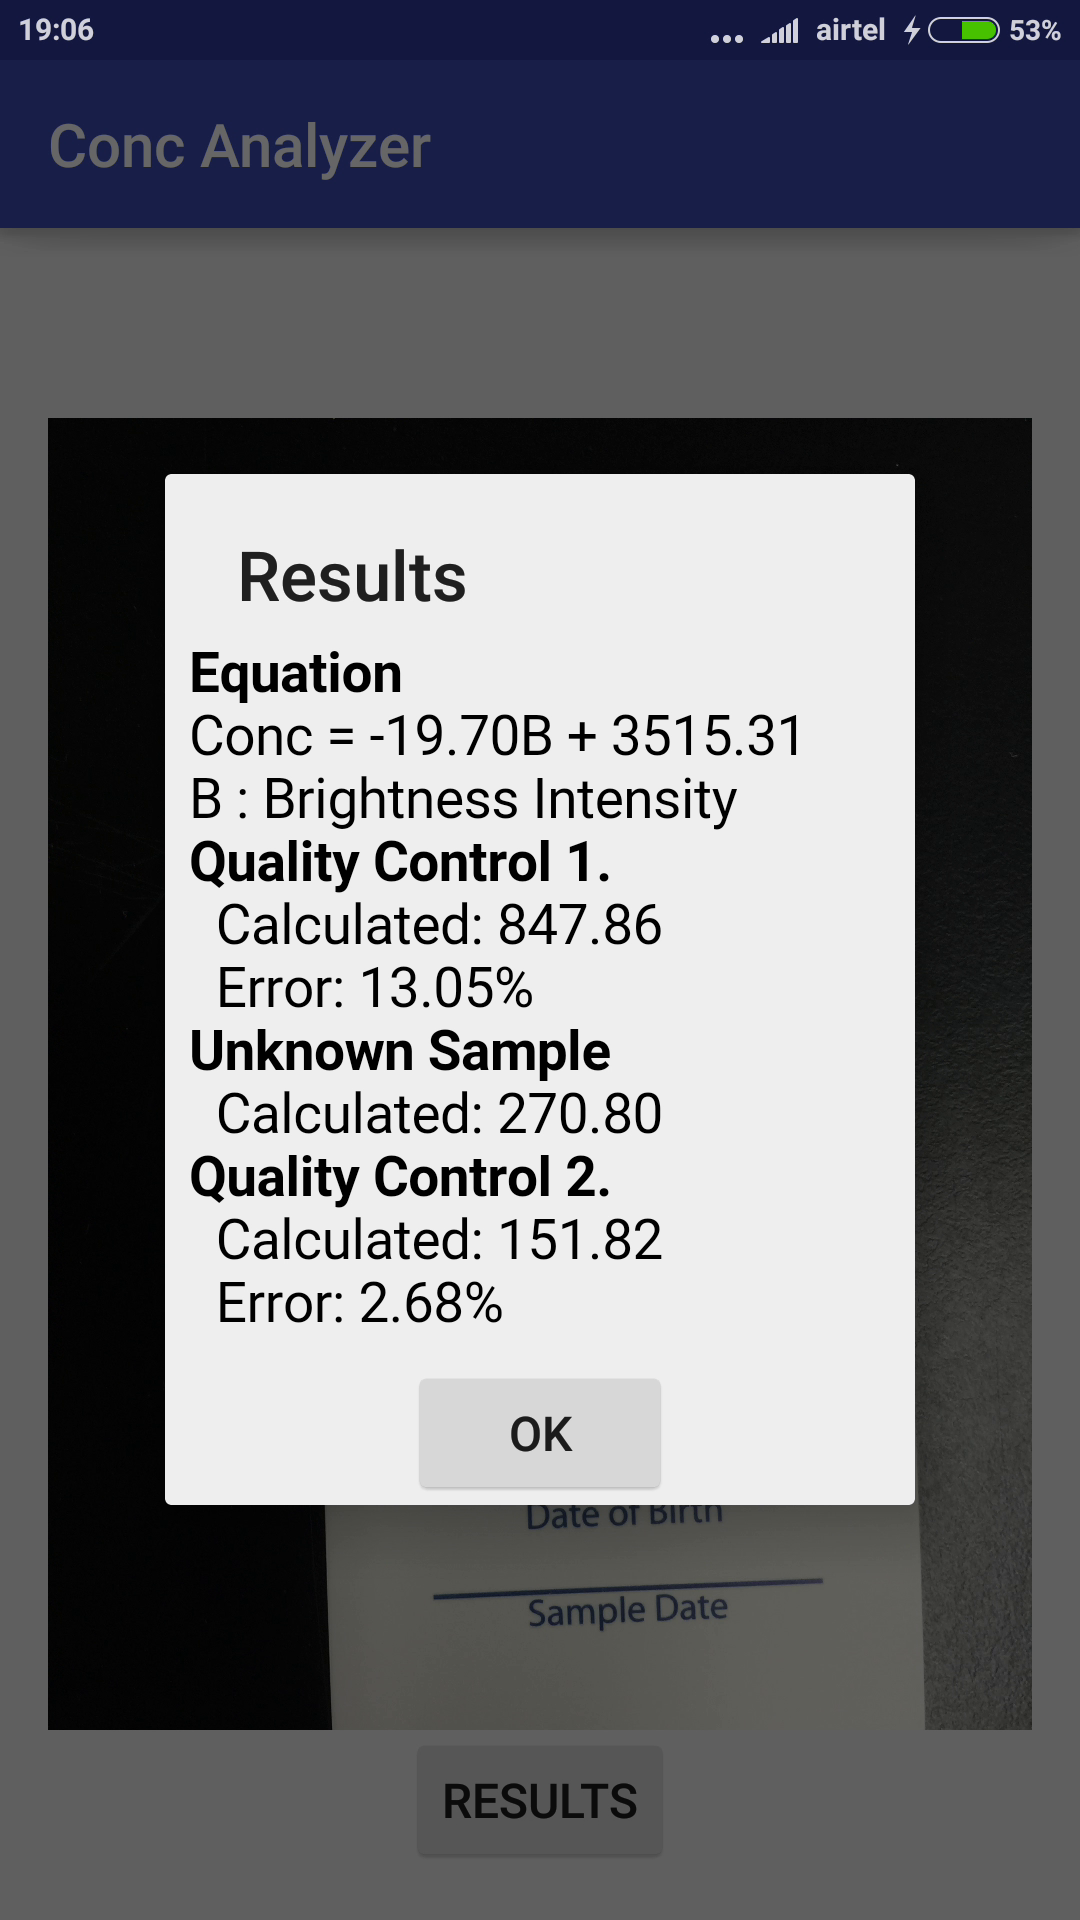
\includegraphics[scale=0.11]{conc6}
\caption{Enter Sample Details \& Results}
\label{fig:scr3}
\end{center}
\end{figure}

\newpage

\section{Project Details}

\subsection{Mobile Based Blood Analysis (Required)}

\textbf{\emph{Skills}}: Java (Android), Image Processing 

\begin{enumerate}
\item \textbf{Image Capture} -- The image containing the blood samples will be captured using the camera package of Android SDK. A guideline image will be overlayed on the camera view to guide the user into taking good quality pictures.
\item \textbf{Segmentation} -- The captured picture will then be segmented using any of the suitable methods (depending on the resultant accuracy of the computation) which include \emph{i) Hue based segmentation}: The image will be converted to $HSV$ color space and segmented based on color bounds of the Hue channel. (This can also be accomplished by converting the image in $YC_{r}C_{b}$ color space and segmenting using $C_{r}$ channel) and \emph{ii) Circle detection based approach}: The edges of input image will be detected using suitable filters (Canny, Sobel etc.) and the circular Hough Transform will be applied on the edge detected image. 
\item \textbf{Noise Reduction} -- The image output from previous step will contain noise and spurious detections. This noise can be completely removed by filtering the image using a 5x5 median filter and then applying morphological operations.
\item \textbf{Detection} -- The blobs which contain the sample can then be detected by finding the contours of the binary image from the previous step and then choosing the largest ones. Since the variation of size of the blobs will be bimodal, the regions of interest can easily be found out by Otsu like method even if the number of samples is unknown. If the number of samples is known, say $N$, the $N$ largest blobs (area wise) will be chosen. The image processing tasks can either be done using OpenCV + JNI as I have done in my prototype or be implemented from scratch, whatever suits the project best. I understand the underlying algorithms perfectly and can efficiently implement them in Java. 
\item \textbf{Measurement} -- The intensities of the detected blobs will be calculated by averaging the intensities of pixels it contains. This can be done by converting the image into grayscale (as I've done in the proposal challenge) or $YC_{r}C_{b}$ or $HSV$ whichever gives the best results.
\item \textbf{Standard Curve Generation \& Estimation} -- A linear curve will be fit through the data using a suitable curve fitting method (least squared error linear regression etc.) and the equation relating the intensity to concentration will be found out. The standard curve will be displayed using suitable graphing API (as I've already done in the \emph{Sanibridge} application) after suitable change of axes along with the equation. The values of unknown samples will be then evaluated from the standard curve and displayed accordingly.

\end{enumerate}

The application will have two modes of processing, \emph{a) Manual Processing} -- where the user will tap on the blobs to add information about them, \emph{b) Batch Processing} -- where the properties of blobs which occur at specific positions will be entered just once and any subsequent images will be processed automatically.

\subsection{REST API \& Web Based Blood Analysis (Optional)}

\textbf{\emph{Skills}}: PHP/Python, C++, HTML+CSS+JS \\

I believe the Android based project won't take much of the time, therefore, I am proposing the following additions to it. 

\begin{itemize}
\item A REST API for performing the same image processing and standard curve estimation tasks online. Since analysis on mobile devices for large images might be a bit time consuming, user will be given a choice to analyze the image online instead (if connected to the internet). The algorithms for this will be rewritten for efficiency and a REST API will be created.
\item A complete Web Application in HTML5 and CSS3 which will use the same backend API. User will be able to upload the image and analyze them interactively. The web application can have two modes namely \emph{a) Automatic} -- where user will upload the image and the analysis will be done automatically, and \emph{b) Expert} -- where user can interact with analysis procedure and choose different methods.

\end{itemize}

\section{Timeline}

\begin{itemize}
\item \textsc{30 April - 22 May}: Familiarize myself with the project problem and prototype different algorithms in Python and C++ to analyze which one gives the best results.
\item \textsc{23 May - 3 June}: Code the best algorithm from the previous step in Android platform and make the first build of application with basic UI structure.
\item \textsc{3 June - 13 June}: Develop the Results section (Standard Curve and Equation) of the application.
\item \textsc{13 June - 21 June}: Make improvements to the user interface and make it intuitive and user friendly. Fix bugs.
\item \textsc{21 June - 28 June}: Mid Term Evaluation Period. Fix Bugs and make general improvements to the application and make the first release build.
\item \textsc{28 June - 8 July}: Develop server backend for allowing user to choose server analysis as an option. 
\item \textsc{8 July - 28 July}: Develop the REST API for the backend server. Develop front end for web application in HTML5, CSS3 and JavaScript.
\item \textsc{28 July - 8 August}: Make changes to the Android application to incorporate server analysis option.
\item \textsc{8 August - 16 August}: Test the Android and Web applications rigorously to fix bugs, if any.
\item \textsc{16 August - 24 August}: Code submission.

\end{itemize}

\section{Questionnaire}

\begin{itemize}
\item Classes \& exams end by 30th April 2016.
\item I don't have any school related activities or internship during summer.
\item I'll be able to work 40 hrs per week on my GSoC project.

\end{itemize}

\section{Why?}

\emph{Why saturation based measurement is best for the task at hand and still I chose not to use it?}\\
When the image is converted into $HSV$ color space and then segmented based on red hue, the next logical step is to measure the intensity by averaging the Saturation of each blob which represents how saturated the blob is with the color red. As the concentration increases, the reddishness i.e. saturation will increase and hence a curve of positive slope will be obtained which will serve as the standard curve. However, in the sample the average saturation value of either C3 or QC1 does not comply with this logic, but this may be due to camera or some other error. Table \ref{table:hsvsat} shows the average saturation values of all samples. The ones which do not comply are in \textcolor{red}{red}. Curve fitting using this data produced results with one calculation breaching the error limit of 20\% so I discarded this method.
\\

\begin{table}
\begin{center}
\setlength\tabcolsep{2.5pt}
\def\arraystretch{1.5}
\begin{tabular}{| m{7em} m{9em} m{9em}|}
\hline
Sample & Concentration & Avg. Saturation\\
\hline
\hline
C2 & 62.5 ng/ml & 31.44\\
\hline
C3 & 125 ng/ml & \textcolor{red}{38.6}\\
\hline
QC1 & 156 ng/ml & \textcolor{red}{33.9}\\
\hline
C4 & 250 ng/ml & 40.5\\
\hline
C5 & 500 ng/ml & 49.5\\
\hline
QC2 & 750 ng/ml & 55.11\\
\hline
C6 & 1000 ng/ml & 56.59\\
\hline

\hline
\end{tabular}
\\
\caption{Saturation based measurement}
\label{table:hsvsat}
\end{center}
\end{table}
\emph{Why is this project important for me?}\\
I'll be going for further studies in the field of Computer Vision. Given my background (Civil Engineering), such a project will be a strong point in my profile and hence I'm passionate about it.\\ \\
\\ \\
\emph{Why should this project be given to me?}\\ 
I'm well-versed in the field of Image Analysis and understand the algorithms to be used perfectly. I'm a research oriented person who is always eager to learn new things, and the project itself aims to provide optimal image analysis results which requires research and trials using various different techniques. 


\end{document}
